\documentclass[11pt]{article}
\usepackage{fullpage,ifthen,enumerate,algo,url}
%\usepackage[pdftex]{graphicx}
\usepackage{graphicx}

\begin{document}
%
% Headings
%
\begin{center}
UNIVERSITY OF WATERLOO\\
Cheriton School of Computer Science\\[\baselineskip]
{\bf CS240\hfill Data Structures and Data Management \hfill
Winter 2013}\\[\baselineskip]
{\sc \large ASSIGNMENT 5}\\
(Due: Monday, April 1, 2013, 9:30am)\\[2\baselineskip]
\end{center}
%
% Main body
%

%\maketitle
\noindent


Please read \url{http://www.student.cs.uwaterloo.ca/~cs240/w13/guidelines.pdf} for
guidelines on submission. Problems 1-3, 4a and 5a are written problems; submit your solutions as PDF files named {\tt a03w.pdf} for all or individual question files named {\tt a03q1w.pdf}, ... , {\tt a03q5aw.pdf}. Implement your programming solutions in C++. Make sure the code you submit runs in the student environment.
\noindent
\begin{enumerate}

\item The worst case of interpolation search results in $\Theta(n)$ search
time. Let $i$ be the interpolated index value as predicted by the formula where
the next comparison in the intepolation search is made. This
splits the array into two parts at least one of which is of length no 
greater than half of the original range. We call this side the ``good side''
while the second part of length at least half the original range is called
the ``bad side''. Assume we keep track of how many times after comparing with
the element $A[i]$ interpolation search recurses on the bad. Let this be a counter called numFailures. A recursion on the ``bad side'' is called an \emph{interpolation
failure}. 

We wish to devise a new formula for the computation of the interpolated index that
pushes the value $i$ in such a way as to make the two parts more balanced, based upon the
number of failures.
\begin{enumerate}
\item {[5 marks]}  Give pseudocode for a modified interpolation search
in which the two parts are made more balanced 
by reducing the size of the larger side by up to the value of numFailures.
Make sure to handle boundary cases.
\item {[5 marks]}  Give the worst case search time for this procedure.
\item {[5 marks]}  Give pseudocode for a modified interpolation search
in which the two parts are made more balanced
by reducing the size of the larger side by up to the value of $2^{\mbox{\small\it numFailures}}$.
Make sure to handle the boundary cases.
\item {[5 marks]} Give the worst case search time for this procedure.
\end{enumerate}


\item {[10 marks]}  
Galloping is sometimes called a one-sided binary search. Describe a one-sided
interpolation search in which instead of searching at locations 1, 2, 4, 8,\ldots
we interpolate (more precisely, extrapolate) 
the next location to be probed on the basis of the ones we
have seen, More specifically, give a formula that computes the index of the
next probe on a one-sided interpolation search which is based on a suitably modified 
interpolation search of the formula seen in class:

\[ i = \ell+\left\lfloor\frac{k-A[\ell]}{A[r]-A[\ell]}(r-\ell)\right\rfloor. \]

\item {[10 marks]}  Implement a procedure called {\tt skipify} which given $n$
 items builds a {\bf deterministic} perfectly balanced skip list with $\lg n$ levels 
 in which exactly every other element from the previous level is promoted to the level 
 above.

\item 	{[5 marks]}
One of the applications of quad trees is compression of pictures. The picture is recursively divided in quadrants until the entire quadrant is of the same colour. Using this rule, draw the quadtree of the following picture.

%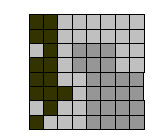
\includegraphics[width=50mm]{image.png} 

\item {[5 marks]} Draw the kd-tree on the points

(1,12) (3,11) (5,10) (7,9) (9,5) (11,6) (13,7) (15,8) 
(2,4) (4,3) (6,2) (8,1) (10,15) (12,14) (14,13) 

\item {[5 marks]} Draw the balanced range tree on the same set of points, i.e.

(1,12) (3,11) (5,10) (7,9) (9,5) (11,6) (13,7) (15,8)
(2,4) (4,3) (6,2) (8,1) (10,15) (12,14) (14,13)


\item {[5 marks]} Senator Raul Payn likes simplistic solutions to complicated problems. He believes
that range trees are a waste of pointers and government money so he chooses to eliminate
the y-coordinate trees and make do with with a balanced BST on the x-coordinates first.
Construct an example of a set of $n$ points and a query rectangle such that the 
(1) the answer is empty and (2) the total number of points examined to answer the
query using an x-coordinate tree is $n$.


\item	{[8 marks]} Consider the Boyer-Moore pattern matching method using only the bad character heuristic as seen in class. Let the alphabet be \verb+{e,f,g,l}+.
    
\begin{enumerate}
\item 	First, compute the shift function for each character of the alphabet over the pattern {\tt gell}
\item	In what follows we show the first few steps of the algorithm, complete the remaining steps to search the entire text. Underline the characters that are compared in each alignment before each shift.

\begin{verbatim}
feelfleeflegellfellgellglee
gell
 gell
\end{verbatim}
\end{enumerate}

\item {[20 marks]}

\begin{enumerate}
\item
	 Show in a diagram the suffix trie for \verb+kneel knell knead keel+.
\item
	 Show in a diagram the suffix trie for \verb+00111000111001$+.
\item
	 Show in a diagram the suffix tree for \verb+kneel keel knell knead+.
\item
	 Show in a diagram the suffix tree for  \verb+00111000111001$+.
\item
 Prove that the suffix trie of a string has $m^2$ nodes when the string is of the form \verb+00...0011...1100...0011...11+ where $m$ is the number of consecutive 0s and 1s.
\end{enumerate}

\item After writing his memoirs, Foghorn Leghorn has decided to compressed them using
      Lempel-Ziv compression with six bit codes.  The code table is initialized only with the codes (a,000000), (b,000001), \ldots, (z,011001) (space, 011010), (', 011011), (, ,011011).  Compress the opening sentence "that's a joke, that's a joke, son, that's a joke".
      
      Given the amount of repetition in the sentence above, comment on the quality of
      compression of LZW in this instance. 
      
      Using the table above decompress 
      
      {\tt 00000000011110010001001000001011011011010010011010000101001110001110001011}
 
\end{enumerate}


\end{document}
